\documentclass[a4 paper]{article}
% Set target color model to RGB



\usepackage[inner=2.0cm,outer=2.0cm,top=2.5cm,bottom=2.5cm]{geometry}
\usepackage{setspace}
\usepackage[rgb]{xcolor}
\usepackage{verbatim}
\usepackage{subcaption}
\usepackage{amsgen,amsmath,amstext,amsbsy,amsopn,tikz,amssymb,tkz-linknodes}
\usepackage{fancyhdr}
\usepackage[colorlinks=true, urlcolor=blue,  linkcolor=blue, citecolor=blue]{hyperref}
\usepackage[colorinlistoftodos]{todonotes}
\usepackage{rotating}
%\usetikzlibrary{through,backgrounds}

\usepackage{lmodern}
\usepackage[T1]{fontenc}
\usepackage[capposition=top]{floatrow}
\usepackage{hyperref}
\usepackage{graphicx}
\graphicspath{ {images/} }
\usepackage{booktabs}
\usepackage{changepage}
\usepackage{float}
\usepackage{fancyvrb}







\hypersetup{%
pdfauthor={Nick Korbit},%
pdftitle={Homework},%
%pdfkeywords={Tikz,latex,bootstrap,uncertaintes},%
pdfcreator={PDFLaTeX},%
pdfproducer={PDFLaTeX},%
}
%\usetikzlibrary{shadows}
% \usepackage[francais]{babel}
\usepackage{booktabs}


\newcommand{\ra}[1]{\renewcommand{\arraystretch}{#1}}

\newtheorem{thm}{Theorem}[section]
\newtheorem{prop}[thm]{Proposition}
\newtheorem{lem}[thm]{Lemma}
\newtheorem{cor}[thm]{Corollary}
\newtheorem{defn}[thm]{Definition}
\newtheorem{rem}[thm]{Remark}
\numberwithin{equation}{section}

\newcommand{\homework}[6]{
   \pagestyle{myheadings}
   \thispagestyle{plain}
   \newpage
   \setcounter{page}{1}
   \noindent
   \begin{center}
   \framebox{
      \vbox{\vspace{2mm}
    \hbox to 6.28in { {\bf ISYE 6420:~Bayesian Statistics \hfill {\small #2}} }
       \vspace{6mm}
       \hbox to 6.28in { {\Large \hfill #1  \hfill} }
       \vspace{6mm}
       \hbox to 6.28in { {\it Instructor: {\rm #3} \hfill Name: {\rm #5}, gtID: {\rm #6}} }
       %\hbox to 6.28in { {\it TA: #4  \hfill #6}}
      \vspace{2mm}}
   }
   \end{center}
   \markboth{#5 -- #1}{#5 -- #1}
   \vspace*{4mm}
}

\newcommand{\problem}[2]{~\\\fbox{\textbf{Problem #1}}\newline\newline}
\newcommand{\subproblem}[1]{~\newline\textbf{(#1)}}
\newcommand{\D}{\mathcal{D}}
\newcommand{\Hy}{\mathcal{H}}
\newcommand{\VS}{\textrm{VS}}
\newcommand{\solution}{~\newline\textbf{\textit{(Solution)}} }

\newcommand{\bbF}{\mathbb{F}}
\newcommand{\bbX}{\mathbb{X}}
\newcommand{\bI}{\mathbf{I}}
\newcommand{\bX}{\mathbf{X}}
\newcommand{\bY}{\mathbf{Y}}
\newcommand{\bepsilon}{\boldsymbol{\epsilon}}
\newcommand{\balpha}{\boldsymbol{\alpha}}
\newcommand{\bbeta}{\boldsymbol{\beta}}
\newcommand{\0}{\mathbf{0}}



%%%%%%%%%%%%%%%%%%%%%%%%%%%%%%%%%%%%%%%%
%%			 Document				  %%
%%%%%%%%%%%%%%%%%%%%%%%%%%%%%%%%%%%%%%%%


\begin{document}
	
\homework{Final Exam}{Spring 2020}{Roshan Vengazhiyil, Brani Vidakovic}{}{Nick Korbit}{903263968}


%%%%%%%%%%%%%%%%%%%%%%%%%%%%%%%%%%%%%%%%
%%			 Problem 1				  %%
%%%%%%%%%%%%%%%%%%%%%%%%%%%%%%%%%%%%%%%%

\problem{1}

Let $y$ be the variable we would like to 
predict -- probability of a person going 
to the beach.
We model $y$ as

\begin{align*}
y_{i}	\sim\mathcal{B}er\left(p_{i}\right) \\
logit\left(p_{i}\right)=\log\frac{p_{i}}{1-p_{i}}=\beta_{0}+\sum_{i=1}^{5}\beta_{i}x_{i}
\end{align*}

We have 5 covariates -- ''Midterm'',  ''Finances'',  
''FriendsGo'',  ''Forecast'' and ''Gender''. 
For each of the covariate coefficients we set a 
flat normal prior with $\mu=0$ and $precision=0.5$. 
So that the OpenBUGS model is 

\begin{Verbatim}
# Training
for (i in 1:n) {
logit(p[i]) <- b0 + b1*Midterm[i] + b2*Finances[i] + b3*FriendsGo[i] 
	+ b4*Forecast[i] + b5*Gender[i]
Beach[i] ~ dbern(p[i])
}

# Priors
b0 ~ dnorm(0.0, 0.5)
b1 ~ dnorm(0.0, 0.5)
b2 ~ dnorm(0.0, 0.5)
b3 ~ dnorm(0.0, 0.5)
b4 ~ dnorm(0.0, 0.5)
b5 ~ dnorm(0.0, 0.5)
\end{Verbatim}

Having trained the model, we would like
to estimate probability distributions 
for Jane, Michael and Melissa.
Knowing the parameters for 
all persons, we specify:

\begin{Verbatim}
jane=c(1,1,0,0,1), michael=c(0,0,1,1,0), melissa=c(1,1,0,1,1)
\end{Verbatim}

And then we proceed to inference:

\begin{Verbatim}
logit(p_jane) <- b0 + b1*jane[1] + b2*jane[2] + b3*jane[3] + b4*jane[4] + b5*jane[5]
logit(p_michael) <- b0 + b1*michael[1] + b2*michael[2] + b3*michael[3] 
	+ b4*michael[4] + b5*michael[5]
logit(p_melissa) <- b0 + b1*melissa[1] + b2*melissa[2] + b3*melissa[3] 
	+ b4*melissa[4] + b5*melissa[5]
\end{Verbatim}

Let's now run an OpenBUGS simulation. We start 
with burning 
the first 10000 observation and update the model 
with the next 100000 samples. First, we plot 
densities for the new points:

\begin{figure}[H]
	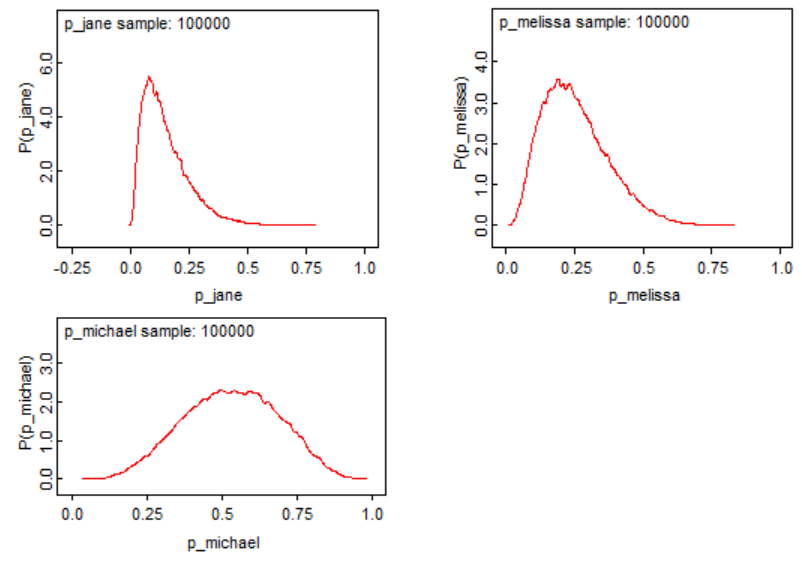
\includegraphics[scale=1.0]{q1}
	\centering
	\label{q1}
\end{figure}

We notice that Jane has the lowest (and most dense) 
probability of going to the beach, with Michael 
having the widest probability density.
Let's now investigate the stats:

\begin{figure}[H]
	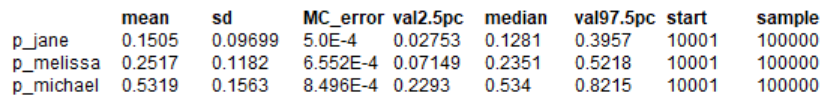
\includegraphics[scale=1.0]{q1_2}
	\centering
	\label{q1_2}
\end{figure}
 
Comparing with the results from the first 
assignment we get:

\begin{figure}[H]
	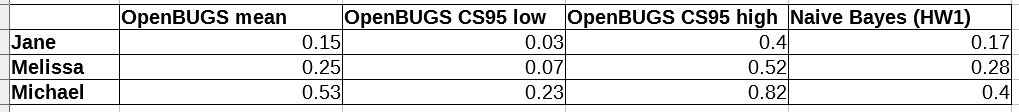
\includegraphics[scale=1.0]{q1_3}
	\centering
	\label{q1_3}
\end{figure}
 
The means of our OpenBUGS simulation are close 
to the original results from Homework 1. All 
original results are within 95\% of
OpenBUGS credible sets. The worst match is for 
Michael, but that's also not surprising 
provided that Michael's probability density is 
the widest.

Note that we should not expect one-to-one
match between OpenBUGS simulation and 
Naive Bayes from HW1 since the model specifications
are different.  \\


\textbf{Note}: the full OpenBUGS code is available 
at \textit{jmmatbeach.odc}
in the attached archive. \\ 

 




%%%%%%%%%%%%%%%%%%%%%%%%%%%%%%%%%%%%%%%%
%%			 Problem 2				  %%
%%%%%%%%%%%%%%%%%%%%%%%%%%%%%%%%%%%%%%%%

\problem{2}

Let $y$ be the variable we would like to 
predict -- the LC50 value. We model $y$ as

\begin{align*}
y_{i}\sim\mathcal{N}\left(\mu,\tau\right)  \\
\mu_{i}=\beta_{0}+\sum_{i=1}^{8}\beta_{i}x_{i}
\end{align*}

We have 8 covariates -- TPSA(Tot) (Molecular properties), SAacc (Molecular properties), H-050 (Atom-centred fragments), MLOGP (Molecular properties), RDCHI (Connectivity indices), GATS1p (2D autocorrelations), nN (Constitutional indices) and C-040 (Atom-centred fragments). 
For each of the covariate coefficients we set a 
normal prior with $\mu=0$ and $precision=0.001$.
We also set a prior for $\tau$ as a gamma distribution
with parameters $(0.001, 0.001)$.
So that the OpenBUGS model is 

\begin{Verbatim}
# Training
for (i in 1:n) {
mu[i] <- b[1] + b[2]*tpsa[i] + b[3]*saacc[i] + b[4]*h050[i] + b[5]*mlogp[i] 
	+ b[6]*rdchi[i] + b[7]*gats1p[i] + b[8]*nn[i] + b[9]*c040[i]
lc50[i] ~ dnorm(mu[i], tau)
}

# Priors
tau ~ dgamma(0.001, 0.001)
for (j in 1:m) {
	b[j] ~ dnorm(0, 0.001)
}
\end{Verbatim}

Next, we specify calculations 
for the new data, both $\mu_{new}$
and $y_{new}$:

\begin{Verbatim}
# Inference
mu_new <- b[1] + b[2]*x[1] + b[3]*x[2] + b[4]*x[3] + b[5]*x[4] 
	+ b[6]*x[5] + b[7]*x[6] + b[8]*x[7] + b[9]*x[8]
lc50_new ~ dnorm(mu_new, tau)
\end{Verbatim}

Let's now run an OpenBUGS simulation. We start 
with burning 
the first 5000 observation and update the model 
with the next 50000 samples. \\

\textbf{a)} First, we plot 
densities for the new points:

\begin{figure}[H]
	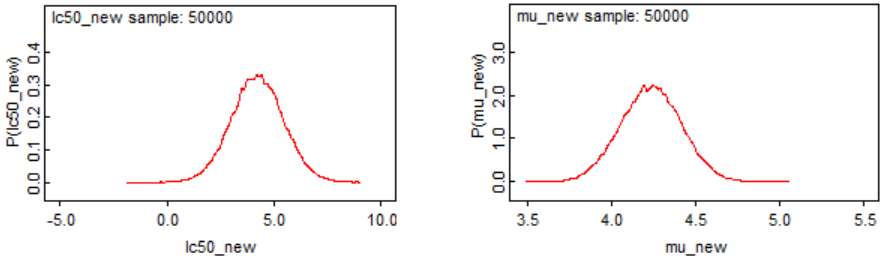
\includegraphics[scale=1.0]{q2}
	\centering
	\label{q2}
\end{figure}

We notice that the density for 
prediction for a new observation
is much more wider than the density for 
the  mean response. We are much more uncertain 
about the actual prediction than $\mu$.
Let's look at the stats:

\begin{figure}[H]
	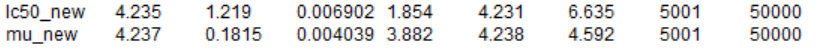
\includegraphics[scale=1.0]{q2_2}
	\centering
	\label{q2_2}
\end{figure}

The means of $\mu_{new}$
and $y_{new}$ are almost the same, however, 
the credible sets are different. For $\mu_{new}$ 
we have a $(3.9, 4.6)$ 95\% set and 
for $y_{new}$ -- $(1.9, 6.6)$. \\


\textbf{b)} Let's now 
analyse the coefficients $\beta_0,..,\beta_8$:

\begin{figure}[H]
	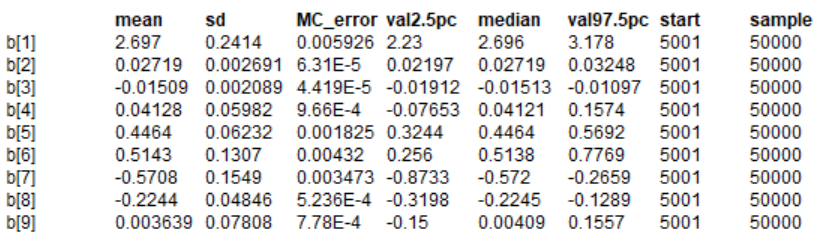
\includegraphics[scale=1.0]{q2_3}
	\centering
	\label{q2_3}
\end{figure}

We notice that $\beta_3$ (b[4]) and $\beta_8$ (b[9])
contain 0 in their respective 95\% 
credible sets. So, we can consider these 
predictors (H-050 and C-040) insignificant 
and exclude them from the model. \\



\textbf{c)} Let's investigate the overall 
quality of the regression by look at 
$R^2$ and $R_{adj}^2$ metrics:

\begin{figure}[H]
	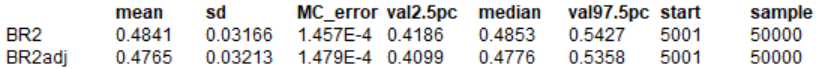
\includegraphics[scale=1.0]{q2_4}
	\centering
	\label{q2_4}
\end{figure}

We see that the overall model quality is 
moderate -- only 0.48. In order to improve 
our model we could do feature engineering
or collect more data. On the feature engineering 
side we can exclude 
the predictors we find insignificant as 
well as modify the existing features (like 
we did it in Assignment 6 with time features).
On the other hand, we could collect more data points
for the same features or include other factors. \\



 

\textbf{Note}: the full OpenBUGS code is available 
at \textit{DaphniaMagna.odc}
in the attached archive. \\ 

%%%%%%%%%%%%%%%%%%%%%%%%%%%%%%%%%%%%%%%%
%%			 Problem 3				  %%
%%%%%%%%%%%%%%%%%%%%%%%%%%%%%%%%%%%%%%%%

\problem{3}

\textbf{a)} In our meta-analysis
we would like to study the effect 
of using amantadine to 
prevent influenza. As a basis for 
the meta-analysis we have the results 
of 8 studies of amantadine 
conducted from 1970 to 1989.

Borrowing from the Blocker OpenBUGS example, 
we assume that in a random effects meta-analysis 
the true effect (on a log-odds scale) $\delta_i$ 
in a trial $i$ is 
drawn from some population distribution.
Let  $r^c_i$ denote the number of cases when 
the subject got influenza in the 
control group 
in trial $i$, and $r^t_i$ denote number of influenza 
cases 
under active amantadine treatment in trial $i$.  
Our model is then:

\begin{align*}
r_{i}^{c}	\sim\mathcal{B}in(p_{i}^{c},n_{i}^{c}) \\
r_{i}^{t}	\sim\mathcal{B}in(p_{i}^{t},n_{i}^{t}) \\
logit(p_{i}^{c})	=\mu_{i} \\
logit(p_{i}^{t})	=\mu_{i}+\delta_{i} \\
\delta_{i}	\sim\mathcal{N}(d,\tau)
\end{align*}


We also specify the model in OpenBUGS terms:

\begin{Verbatim}
# Training
for(i in 1:n) {
	# Placebo
	rc[i] ~ dbin(pc[i], nc[i])
	logit(pc[i]) <- mu[i]
	mu[i] ~ dnorm(0.0, 0.00001)
	
	# Drug
	rt[i] ~ dbin(pt[i], nt[i])
	logit(pt[i]) <- mu[i] + delta[i]
	delta[i] ~ dnorm(d, tau)
}
\end{Verbatim}

We set uniformative priors for 
all variables:

\begin{Verbatim}
d ~ dnorm(0.0, 0.000001)
tau ~ dgamma(0.001, 0.001)
\end{Verbatim}

And run the simulation.
We start 
with burning 
the first 5000 observation and update the model 
with the next 50000 samples.
We then investigate the 
densities for $\delta$ and its 
mean $d$ and variace $\sigma$:

\begin{figure}[H]
	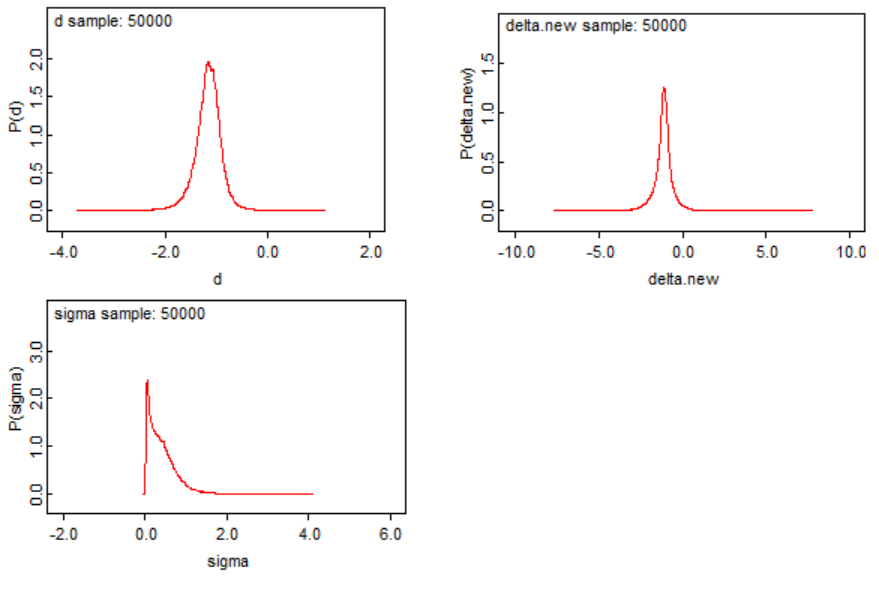
\includegraphics[scale=1.0]{q3}
	\centering
	\label{q3}
\end{figure}

Visually we notice that the mean 
of $\delta$ is tightly distributed 
around $-1$, so we might conclude
that amantadine indeed causes the
descrease in influenza cases.

Let's look at the stats:

\begin{figure}[H]
 	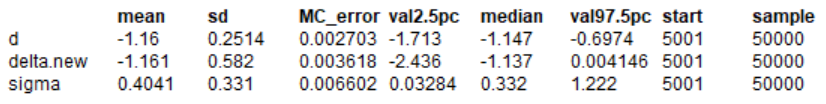
\includegraphics[scale=1.0]{q3_1}
 	\centering
 	\label{q3_1}
\end{figure}

We see that the mean of $d$ is $-1.16$
with 95\% credible set of $(-1.71, -0.70)$.
That clearly points to the effectiveness 
of amantadine. However, the distribution 
for $\delta$ is wider, with 95\% credible set
of $(-2.44, 0.004)$. Although the right 
tail is slightly greater than $0$ we still 
believe that the posterior shows the 
effectiveness of the drug.

Why do we use Bayesian analysis instead
of conventional meta-analysis 
(eg. as specified in \cite{col})?
We could find several reasons \cite{bma}:

\begin{itemize}
\item By modeling $\tau$ the Bayesian meta-analysis 
takes into account the uncertainty
around the heterogeneity variance;

\item Posterior distribution for $\tau$ makes heterogeneity 
evaluation
and investigation more reliable;

\item We could perform sensitivity analysis by changing
distributional assumptions and incorporating 
a priori knowledge into the model (it's a bit hack-ish way,
but we could make the right tail of the 95\% 
credible set for $\delta$ be less than $0$ by 
tweaking the priors);

\item We could add complexity by 
making a deep hierarchical Bayes model.
\end{itemize} 




\textbf{b)} A good overview of the 
meta-analysis visualization toolbox
is made by Kiran et al (2016) \cite{card}.
The authors define 2 main charts for 
meta-analysis -- a forest plot
and a funnel plot.
With the forest plot we investigate the parameter 
estimates of each study and the overall pooled
estimate. 
The funnel plot is a scatter plot, where each dot represents an
individual study and is positioned according to its effect size or
strength of association (x-axis) and the precision around its estimate (y-axis) \cite{card}.

Let's build both plots for our influenza 
data with a Python library
PyMeta \cite{pymeta}. We start with a forest plot:

\begin{figure}[H]
	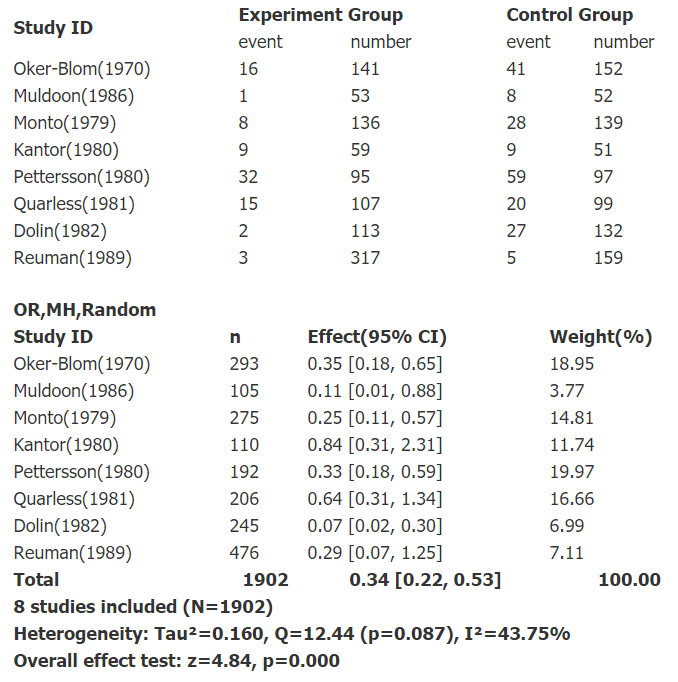
\includegraphics[scale=0.7]{q3_4}
	\centering
	\label{q3_4}
\end{figure}

\begin{figure}[H]
	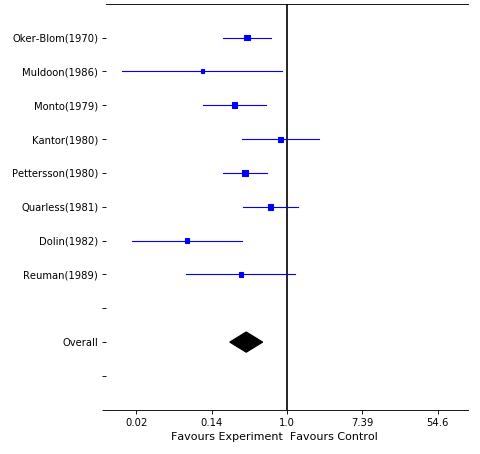
\includegraphics[scale=0.7]{q3_2}
	\centering
	\label{q3_2}
\end{figure}

The squares on our chart show the weight 
given to each study -- the larger the square 
the bigger the weight. The pooled effect 
is denoted by a diamond. In our case all 
the studies and the cumulative effect 
favour the amantadine treatment. 
We also notice that the studies that 
favour amantadine most are Muldoon(1986)
and Dolin(1982). However, those are also 
the studies that have longer
confidence intervals (represented by horizonatal lines).
The studies which confidence intervals 
cross the vertical lines
(in our case Kantor(1980), Quarless(1981) 
and Reuman(1989)) are deemed 
inconclusive.


Then we build a funnel plot:

\begin{figure}[H]
	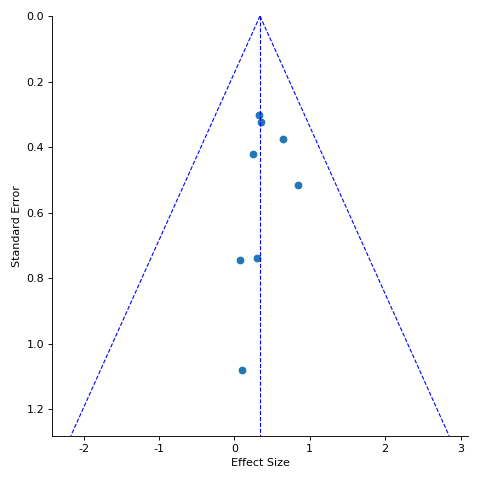
\includegraphics[scale=0.6]{q3_3}
	\centering
	\label{q3_3}
\end{figure}

We see that our funnel chart is symmetric
with all points located inside the triangle.
We might expect the lower points to be 
more widely spread (i.e. results from smaller 
studies tend to deviate from the average), 
however, that's not the case for the 
influenza data.
So we can conclude that the 
data is ``well-behaved'' with no publication bias.  \\

\textbf{Note}: the full OpenBUGS code is available 
at \textit{Influenza.odc} in the attached archive,
the python code for generating plot 
is named \textit{plot\_q3.py} and could be 
run by \textit{python3 plot\_q3.py} command.  \\ 


%%%%%%%%%%%%%%%%%%%%%%%%%%%%%%%%%%%%%%%%
%%			 Bibliography			  %%
%%%%%%%%%%%%%%%%%%%%%%%%%%%%%%%%%%%%%%%%

\begin{thebibliography}{9}


\bibitem{stat}\label{stat} 
Engineering Biostatistics: An Introduction using MATLAB and WinBUGS. 
Brani Vidakovic -- Wiley Series in Probability and Statistics.


\bibitem{col}\label{col} 
Introduction to Meta-Analysis --
Charles DiMaggio. \url{http://www.columbia.edu/~cjd11/charles_dimaggio/DIRE/resources/Bayes/Bayes4/metaAnalysis2011.pdf}


\bibitem{bma}\label{bma} 
Bayesian Meta-Analysis. \url{https://e-l.unifi.it/pluginfile.php/371990/mod_resource/content/1/Meta-analisi_lezione2.pdf}

\bibitem{card}\label{card} 
Graphics and Statistics for Cardiology: Data visualisation for meta-analysis. \url{https://heart.bmj.com/content/103/1/19.full}

\bibitem{pymeta}\label{pymeta} 
PythonMeta library for visualizing meta-analysis. \url{https://www.pymeta.com/help/#pythonmeta}




\end{thebibliography}



\end{document} 